\section{Indgangsvælger}
\label{indgangsvaelger}
Der vil i dette afsnit blive gennemgået de overvejelser gruppen har gjort sig omkring indgangsvælgeren. Der er i kravspecifikationen stillet en række krav som indgangsvælgeren minimum skal overholde. Der vil blive designet ud fra disse krav og afsnittet munder ud i at indgangsvælgeren til HiFi-forstærkeren laves.

\begin{figure}[h]
\centering
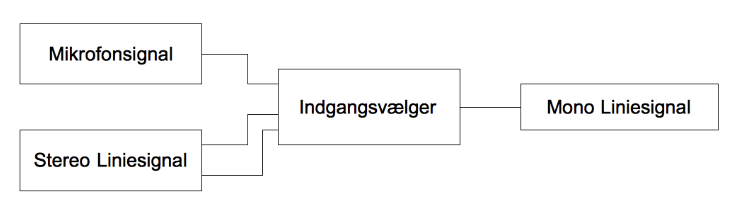
\includegraphics[scale=0.4]{implementering/indgangsvaelger/overordnetdesign.png}
\caption{Blokdiagram over indgangsvælgeren og dens funktioner.}
\label{indgangsvaelger-overordnet}
\end{figure}

Indgangsvælgeren skal håndtere 3 liniesignaler i form af et mikrofonsignal og et liniesignal i stereo. Fra kravspecifikation ved vi at indgangsvælgeren skal være trinvis med 3 trin, og at isoleringen mellem signaler skal være mere end 60 dB. ud over dette skal indgangsvælgeren også være i stand til at samle alle inputsignaler til et udgangssignal. For at gøre det nemmere at overskue er der valgt at opdele indgangsvælgeren i to dele. Første del er isoleringen af signaler, og den anden er Summationen af signaler.

\subsection*{Isolering af Signaler}

\subsection*{Summation af signaler}




